\documentclass[letterpaper,12pt]{article}
\renewcommand{\baselinestretch}{1.5}
\renewcommand*\footnoterule{}
\usepackage{times}
\usepackage[margin=1in]{geometry}
\newcommand*\apostrophe{\textsc{\char39}}
\setlength{\paperheight}{11in}
\setlength{\paperwidth}{8.5in}
\usepackage{graphicx}
\DeclareGraphicsExtensions{.pdf,.jpeg,.png}
\usepackage{cite}
\usepackage{amsmath}
\usepackage{titlesec}
\titlelabel{\thetitle.\quad}
\titleformat*{\section}{\normalfont\bfseries}
\titleformat*{\subsection}{\normalfont\bfseries}
\titleformat*{\subsubsection}{\normalfont\bfseries}
\titleformat*{\paragraph}{\normalfont\bfseries}
\titleformat*{\subparagraph}{\normalfont\bfseries}


\usepackage[numbers,sort&compress]{natbib}

\usepackage{color}
\renewcommand{\bibfont}{\footnotesize}

%\usepackage{hyperref}
%\usepackage{hypernat}
\usepackage{cite}
%\usepackage{hyperref}
\usepackage{url}
\usepackage{multicol}  
\usepackage{multirow}
\usepackage{booktabs}  
\usepackage{threeparttable}
\usepackage{hyperref}
\usepackage{indentfirst}  

\usepackage{color}
\usepackage{graphicx}
\usepackage{subfigure}

\usepackage{amsmath,amssymb,amsfonts}
\usepackage{algorithmic}

\usepackage{algorithmic,algorithm}
\renewcommand{\algorithmicrequire}{\textbf{Input:}}
\renewcommand{\algorithmicensure}{\textbf{Output:}}
\newtheorem{theorem}{Theorem}
\newtheorem{lemma}{Lemma}
\newtheorem{remark}{Remark}
\newtheorem{proposition}{Proposition}
\newtheorem{corollary}{Corollary}
\renewcommand{\algorithmicrequire}{\textbf{Input:}}
\renewcommand{\algorithmicensure}{\textbf{Output:}}
\renewcommand{\thefootnote}{\alph{footnote}}  

\begin{document}
\date{}

\title{FLOWGAN: DEEP LEARNING BASED ENCRYPTED NETWORK TRAFFIC CLASSIFICATION WITH CLASS IMBALANCE }
\author{Pan Wang$^{1}$ , ZiXuan Wang $^{1}$ , ShuHang Li $^{1}$ , Chen Huang $^{1}$ ,Feng Xiang $^{2}$
   \and
   $^{1}$ School of Modern Posts, University of Nanjing University \\ of Posts and Telecommunications, Nanjing,CO 210003, China
   \and
   $^{2}$ YTO Express Co., Ltd., Shanghai,CO 201705,China
   \and
    Corresponding author: Pan Wang (e-mail: wangpan@njupt.edu.cn)
}


% The following lines should be within the Author's block
%\footnote{Manuscript received December 15, 2015} 

%Authors' information should be left commented for the submittal of the %manuscript.  The comments should be removed for the final submittal
%FirstName LastName \\
%Department of XXXXXXXXXX\\
%University of XXXXXX\\
%Address1\\
%City, State, ZIP, Country \\
%email: email@address.com \\
%\and
%FirstName LastName \\
%Department of XXXXXXXXXX\\
%University of XXXXXX\\
%Address1\\
%City, State, ZIP, Country \\
%email: email@address.com \\
%\and
%FirstName LastName \\
%Department of XXXXXXXXXX\\
%University of XXXXXX\\
%Address1\\
%City, State, ZIP, Country \\
%email: email@address.com \\

\maketitle

\thispagestyle{empty}

\noindent
{\bf\normalsize Abstract}\newline
{It is crucial to accurately identify the type of traffic and application so that it can enable various policy-driven network managements and security monitoring. However, with more and more adoptions of encryption over internet applications, it brings a lot of challenges about traffic classification. Although classical machine learning approaches and recent proposed deep learning methods can solve many issues that port and payload based methods cannot solve, it still has some limitations, one of which is imbalanced property of network traffic data. In this paper, we proposed a deep learning method called FlowGAN to tackle with the problem of class imbalance for traffic classification. As an instance of Generative Adversarial Network (GAN), FlowGAN leverages the superority of GAN's data augmentation to generate synthesized traffic data samples for minor classes.  Furthermore, we trained a classical deep learning model, Multilayer perceptron (MLP) based network traffic classifier to evaluate the performance of FlowGAN. Based on public dataset 'ISCX', our experimental results show that our proposed FlowGAN can outperforms unbalanced dataset and balancing dataset by oversampling method in terms of data augmentation. } \vspace{2ex}
   
\noindent
{\bf\normalsize Key Words}\newline
{traffic classification, encrypted traffic, deep learning, Generative Adversarial Network, class imbalance}

\section{Introduction}
Network traffic identification and classification is an important research topic in the field of network management and security. Efficient, accurate and real-time traffic classification is of great practical significance to provide service quality assurance, dynamic access control and abnormal network behaviors detection. However, with the widespread adoptions of encryption techniques in internet applications, encrypted traffic has dramatically become a great challenge for network management and security monitoring.

Traditionally, the evolution of encrypted traffic classification technology has gone through three stages: port-based, payload-based and flow-based statistical characteristics. Port-based classification method infers application's type by assuming that most applications consistently use 'well known' TCP or UDP port numbers, however, the emergence of port camouflage, random port and tunneling technology makes these methods lose efficacy quickly. Payload-based methods, namely, DPI (Deep Packet Inspection) technology cannot deal with encrypted traffic because they need to match packet content and have high computational overhead~\cite{SDN-HGU,PhoneNumber}. As a result, in order to attempt to solve the problem of encrypted traffic identification , flow-based methods emerged, which usually rely on statistical or time series features and employ Machine Learning (ML) algorithms,  such as naive bayes(NB), support vector machine(SVM), decision tree, Random Forest(RF), k-nearest neighbor(KNN) ~\cite{Pescape2008}. Although classical machine learning approach can solve many issues that port and payload based methods cannot solve, it still has some limitations, such as handcrafted traffic features driven by domain-expert, time-consuming, unsuited to automation, rapidly outdated when compared to the evolution. Unlike most traditional ML algorithms, Deep Learning performs automatic feature extraction without human intervention, which undoubtedly makes it a highly desirable approach for traffic classification, especially encrypted traffic.  Recent research work has demonstrated the superiority of DL methods in traffic classification~\cite{MobileTC-2018}, such as MLP, CNN, SAE, LSTM. 


However, imbalanced class distribution of a dataset has posed a serious difficulty to most classifiers based on machine learning algorithms which assume a relatively balanced distribution~\cite{Japkowicz:2002}. Imbalanced class distribution is characterized as that there are many more instances of some classes than others. Network traffic classification is no exception due to the imbalanced property of network traffic data~\cite{Vu2017}. Therefore, how to overcome the problem of imbalanced class distribution in traffic dataset  plays a very crucial role in the network traffic classification. However, very few research has been conducted focusing on examining the performance of traffic classification when facing the problem of imbalanced traffic data, especially deep learning methods.

In this paper, we present the design and development of Generative Adversarial Network (GAN) based traffic data augmenting method called FlowGAN to generate synthesized samples for encrypted traffic classification. The synthesized data is then combined with the original (viz. real) data to construct the new traffic training dataset. As a proof of concept, we adopted three state-of-the-art deep learning based encrypted traffic classification methods, MLP on our new augmented training dataset synthesized from our FlowGAN. The experimental results demonstrate that our proposed FlowGAN can achieve better performance compared with  other traditional data augmenting methods like over sampling~\cite{ROS2004}.

The rest of this paper is organized as follows. Section II introduces the preliminaries and related works of traffic classification, some current methods for tackling with the problem of imbalanced class data and GAN. Section III illustrates the algorithm of GAN and application of generating traffic samples. Section IV describes the methodology of FlowGAN. The experimental results are provided and discussed in Section V. Section VI  concludes our work and presents some future works.
 


\section{Related works}\label{sec:preliminaries}
\subsection{Deep Learning based Traffic Classification}
Traffic classification has play a crucial role in the network management  domain, especially QoS. In summary, there are three approaches to identify network traffic: port-based, payload-based and machine learning based. Unlike most traditional ML algorithms, Deep Learning performs automatic feature extraction without human intervention, which undoubtedly makes it a highly desirable approach for traffic classification, especially mobile services encrypted traffic. Recent research work has demonstrated the superiority of DL methods in traffic classification~\cite{MobileTC-2018,Datanet,Wang-1D-CNN,IoT-CNN-2017,HierarchicalTC}. The application of DL techniques involves three steps. First, model inputs are defined and designed according to some principles, such as packets, PCAP files, flow statistics vectors. Second, models and algorithms are deliberately chosen based on models' characteristics and aim of the classifier. Finally, the DL classifier is trained to automatically extract the features of traffic and associate the inputs with corresponding class labels.

\subsection{Methods for handling imbalanced data}
Generally, there are three approaches for tackling with imbalanced data: \emph{\textbf{Modifying the objective cost function, Sampling and Generating artificial data}}~\cite{Vu2016}. The approach of \emph{\textbf{modifying objective cost function}} alleviates the problem of class imbalance by means of weighting the data samples in minor and major classes differently, which gives higher score on the minor samples to penalize more intensely on miss-classifiying of the sample in the minor class. Sampling methods include two different ways of \emph{\textbf{under-sampling}} and \emph{\textbf{over-sampling}}, which to reduce the size of major class by removing some major data samples and raising the samples in the minor class, respectively. Random under sampling (RUS) and Random over sampling (ROS) are two main methods of under-sampling and over-sampling~\cite{ROS2004}. RUS randomly removes some instances in major class, accordingly, ROS generates some copies of samples of the minor class. However, overfitting problem is always the main drawback of ROS due to generating same copies from the minor class. A classical method for generating artificial data is Synthetic Minority Over-sampling Techinique (SMOTE) in which minority samples are generated by synthetic samples rather than copies~\cite{SMOTE2002}.


\section{GAN}
\subsection{Overview of GAN}
Generative adversarial network(GAN) has been considered as a promising technique since proposed by Goodfellow in 2014~\cite{GAN2014}, which is a framework to train the generative models. The main idea of GAN is that two networks, the generator network and discriminator network, play a minimax game in order to converge to an optimal solution. GAN has shown its state-of-the-art advance in the generation of images, sound and texts. A basic architecture of GAN is shown in Fig.~\ref{fig:basicGAN}. To learn the generator's distribution $G(z)$, a prior on input noise variables $p_z(z)$ is defined. Meanwhile, discriminator's distribution $D(x)$ is defined, which represents the probability that $x$ comes from the real data repository  represented by $p_{data}(x)$ rather than $G(z)$. One can train $D$ to maximize the probability of assigning the correct label to both training examples and samples from $G$ by fine tuning, which is trained to minimize $log(1-D(G(z)))$. In summary, $D$ and $G$ play the following two-player minimax game with value function $V(D,G)$, which is shown as following (~\ref{equ:GAN}):

\begin{figure}[!t]
	\centering
	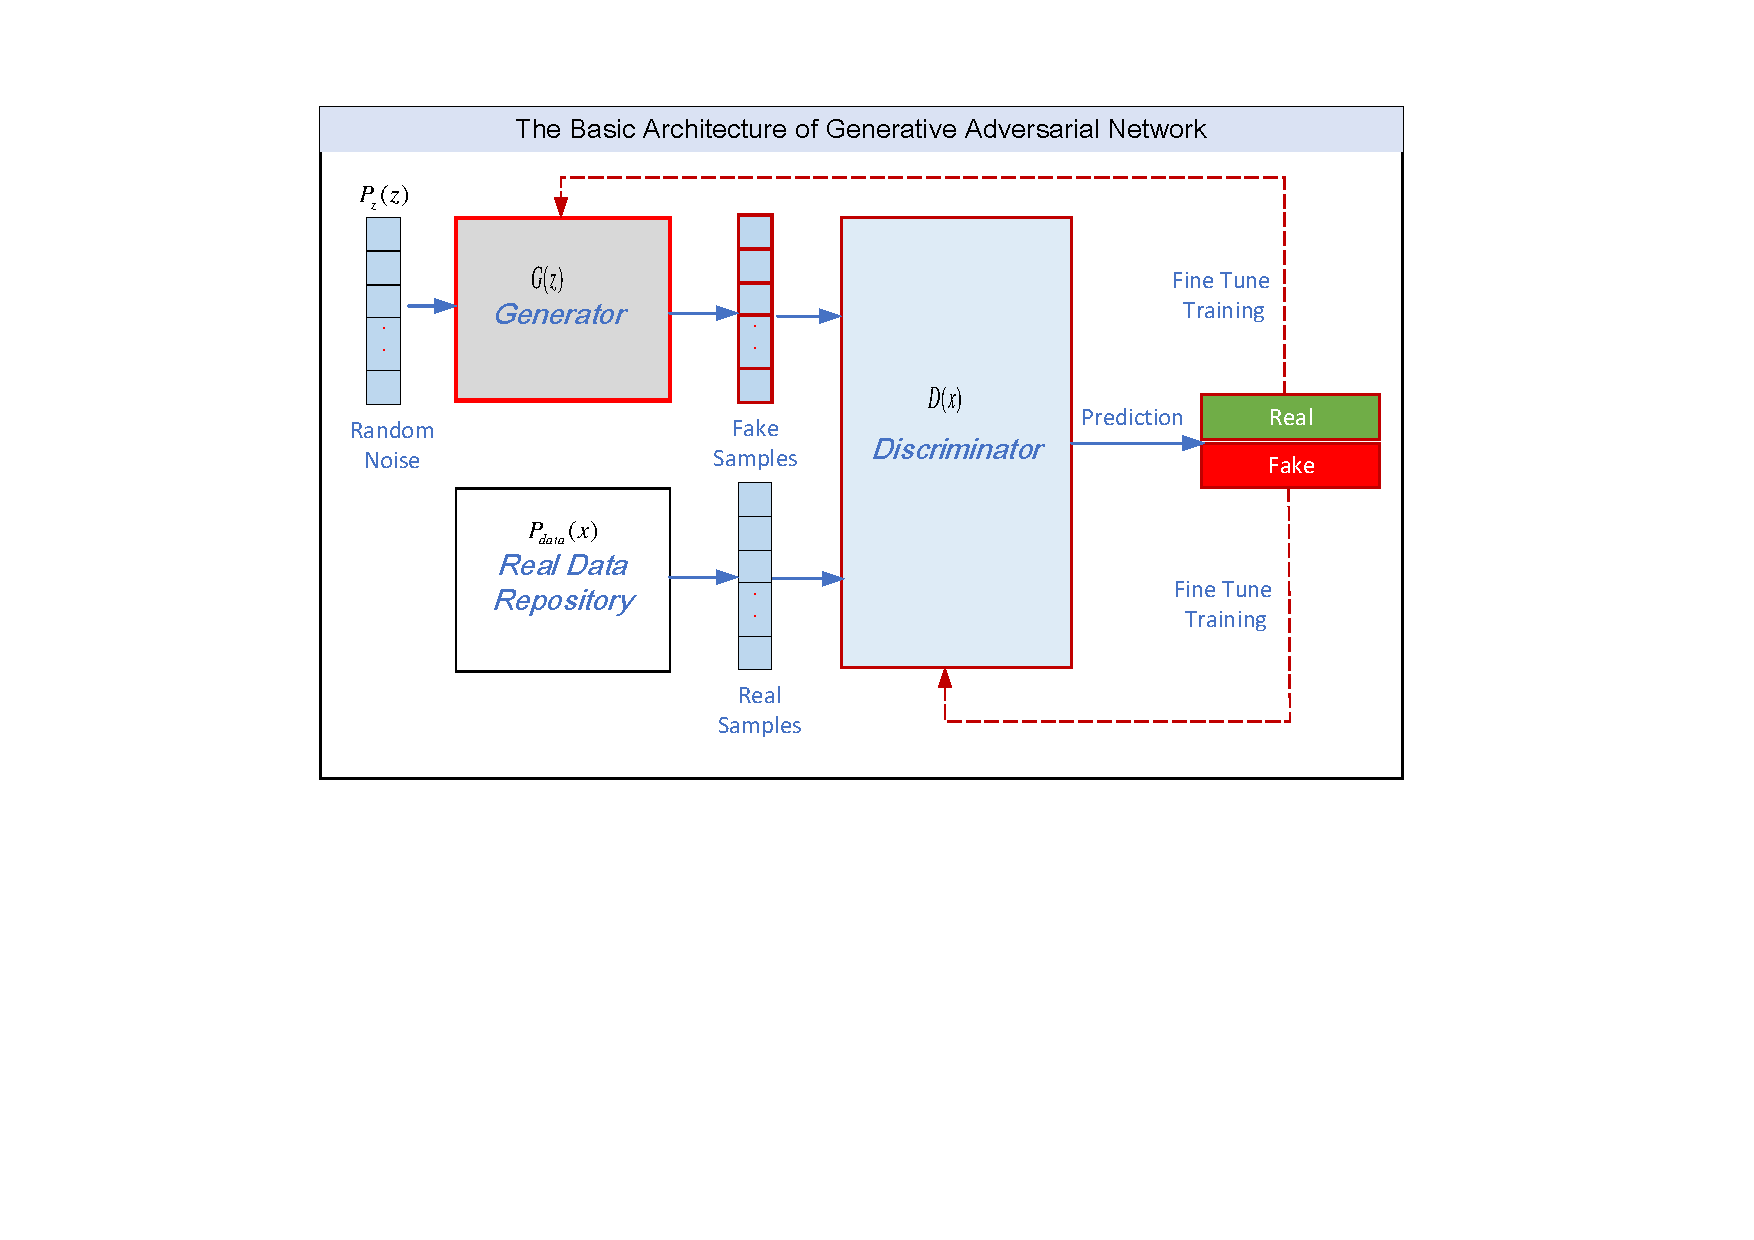
\includegraphics[width=6 in]{figures/Fig_1_basicGAN}
	\caption{The basic architecture of GAN}
	\label{fig:basicGAN}
\end{figure}

%Equations are automatically numbered
\begin{equation}
	\mathop {\min }\limits_{\rm{G}} \mathop {\max }\limits_D V(D,G) = \mathbb{E}_{x\sim{p_{data}}(x)}[\log D(x)] + {\mathbb{E}_{z\sim{p_z}(z)}}[\log (1 - D(G(z)))]
	\label{equ:GAN}
\end{equation}

The generator $G$ takes random noise as input and generates fake samples. The discriminator $D$ is fed with samples from both the generator and the real training data and attempt to distinguish between the two sources. These two networks play a competitive game, where the generator $G$ is learning to generate more and more realistic samples, and the discriminator $D$ is learning to get better and better at distinguishing the generated data from the real data. These two networks are trained simultaneously, and hope that the competition will drive the generated samples to be indistinguishable from the real data. The output of the generator $G$ is a synthesized sample $X_{fake} = G(z)$. Discriminator network $D$ takes the input of a real data sample or a synthesized sample from the generator and the output is a probability distribution $P(F|X) = D(X)$ over possible sources. Discriminator $D$ is trained to maximize the log-likelihood to assigns the correct label as shown in equation (~\ref{equ:fake}) while Generator $G$ is trained to minimize the second term in this equation.

\begin{equation}
L{\rm{ = }}E[\log P(F = real|{X_{real}})] + E[\log P(F = fake|{X_{fake}})
\label{equ:fake}
\end{equation}




\subsection{The application of GAN in generating traffic data samples}
Similar with texts or sentences, GAN can also be applied to the traffic data generation. Current researches have shown that GAN can improve the malware detection or IDS~\cite{Hu2017GAN}. As for the application of GAN in the traffic classification, recent research work has proposed some ideas using GAN to generate the traffic samples to overcome the imbalaced property of network data. In~\cite{Vu-GAN}, the authors adopted an unsupervised learning method called auxiliary classifier GANs(AC-GAN) to generate synthesized traffic samples for balancing between the minor and major classes over a well-known traffic dataset NIMS which only included SSH and non-SSH two classes. The AC-GAN took both a random noise and a class label as input in order to generate the samples of the input class lable accordingly. The experimental results have shown that their proposed method achieved better performance compared to other methods like SMOTE. 


\section{FlowGAN - GAN based traffic data generating method}\label{sec:flowgan}

\subsection{The Framework of FlowGAN Based Encrypted Traffic Classification}
This section will discuss the framework of FlowGAN based encrypted traffic classification shown in Fig.~\ref{fig:framework_gan}. The same as general architecture of deep learning based traffic classification, there are six steps for traffic classification, which is  classification task definition, data preparation, data pre-processing, model input design, pre-training design, model architecture design. The detail has been introduced in our previous work~\cite{TC-DL-Survey}. Apparently, the only difference between FlowGAN based framework and general architecture is data augmentation in data preparation phase. FlowGAN proposed by us is the method of data augmentation to alleviate the problem of imbalanced class data.

\begin{figure}[!t]
	\centering
	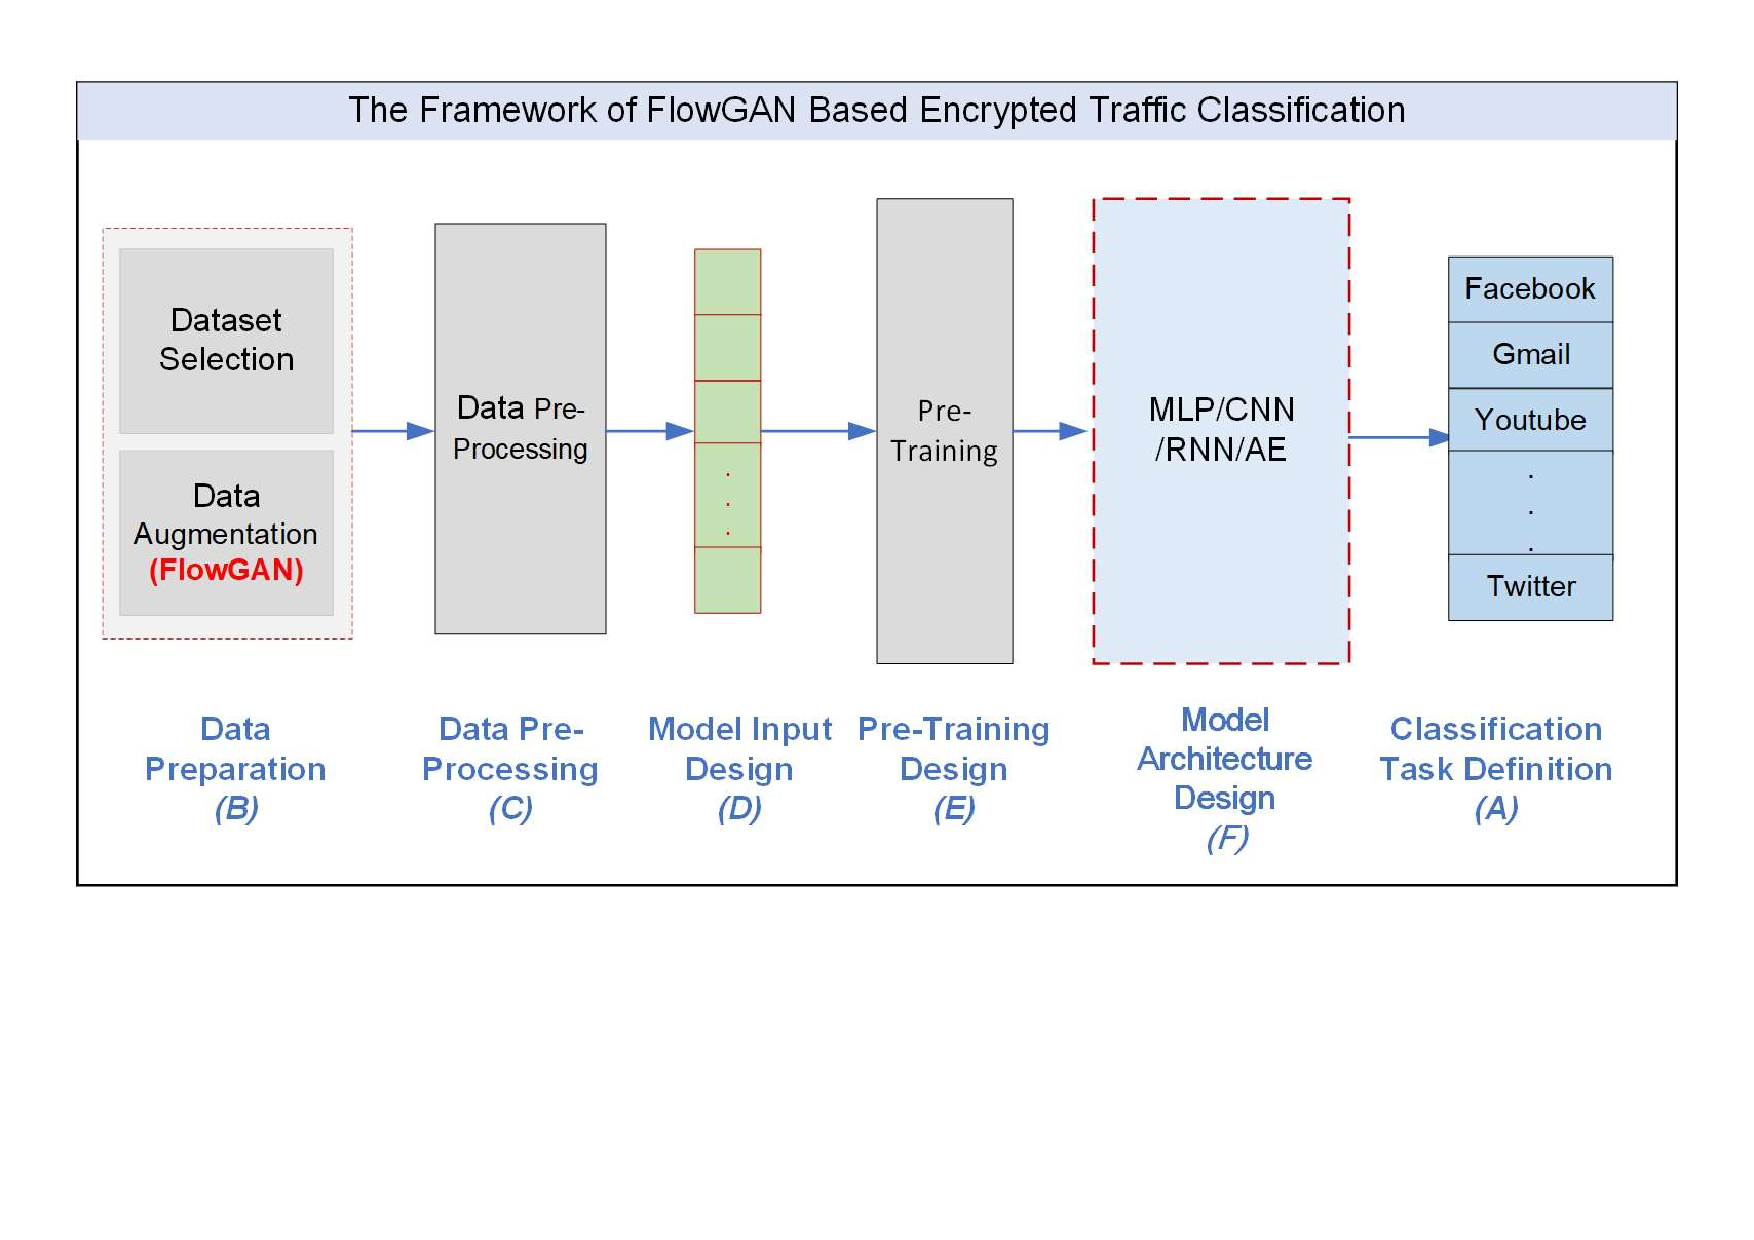
\includegraphics[width=6 in]{figures/Fig_2_flowgan_framework}
	\caption{The framework of FlowGAN based encrypted traffic classification}
	\label{fig:framework_gan}
\end{figure}


\subsection{The Methodology of FlowGAN}
The methodology of FlowGAN is shown in Fig.~\ref{fig:methodology_gan}. There are three phases during the traffic data generating by FlowGAN, which are raw PCAP files pre-processing, GAN model training and data balancing. The detail of each phase will be illustrated as follows.

\begin{figure}[!t]
	\centering
	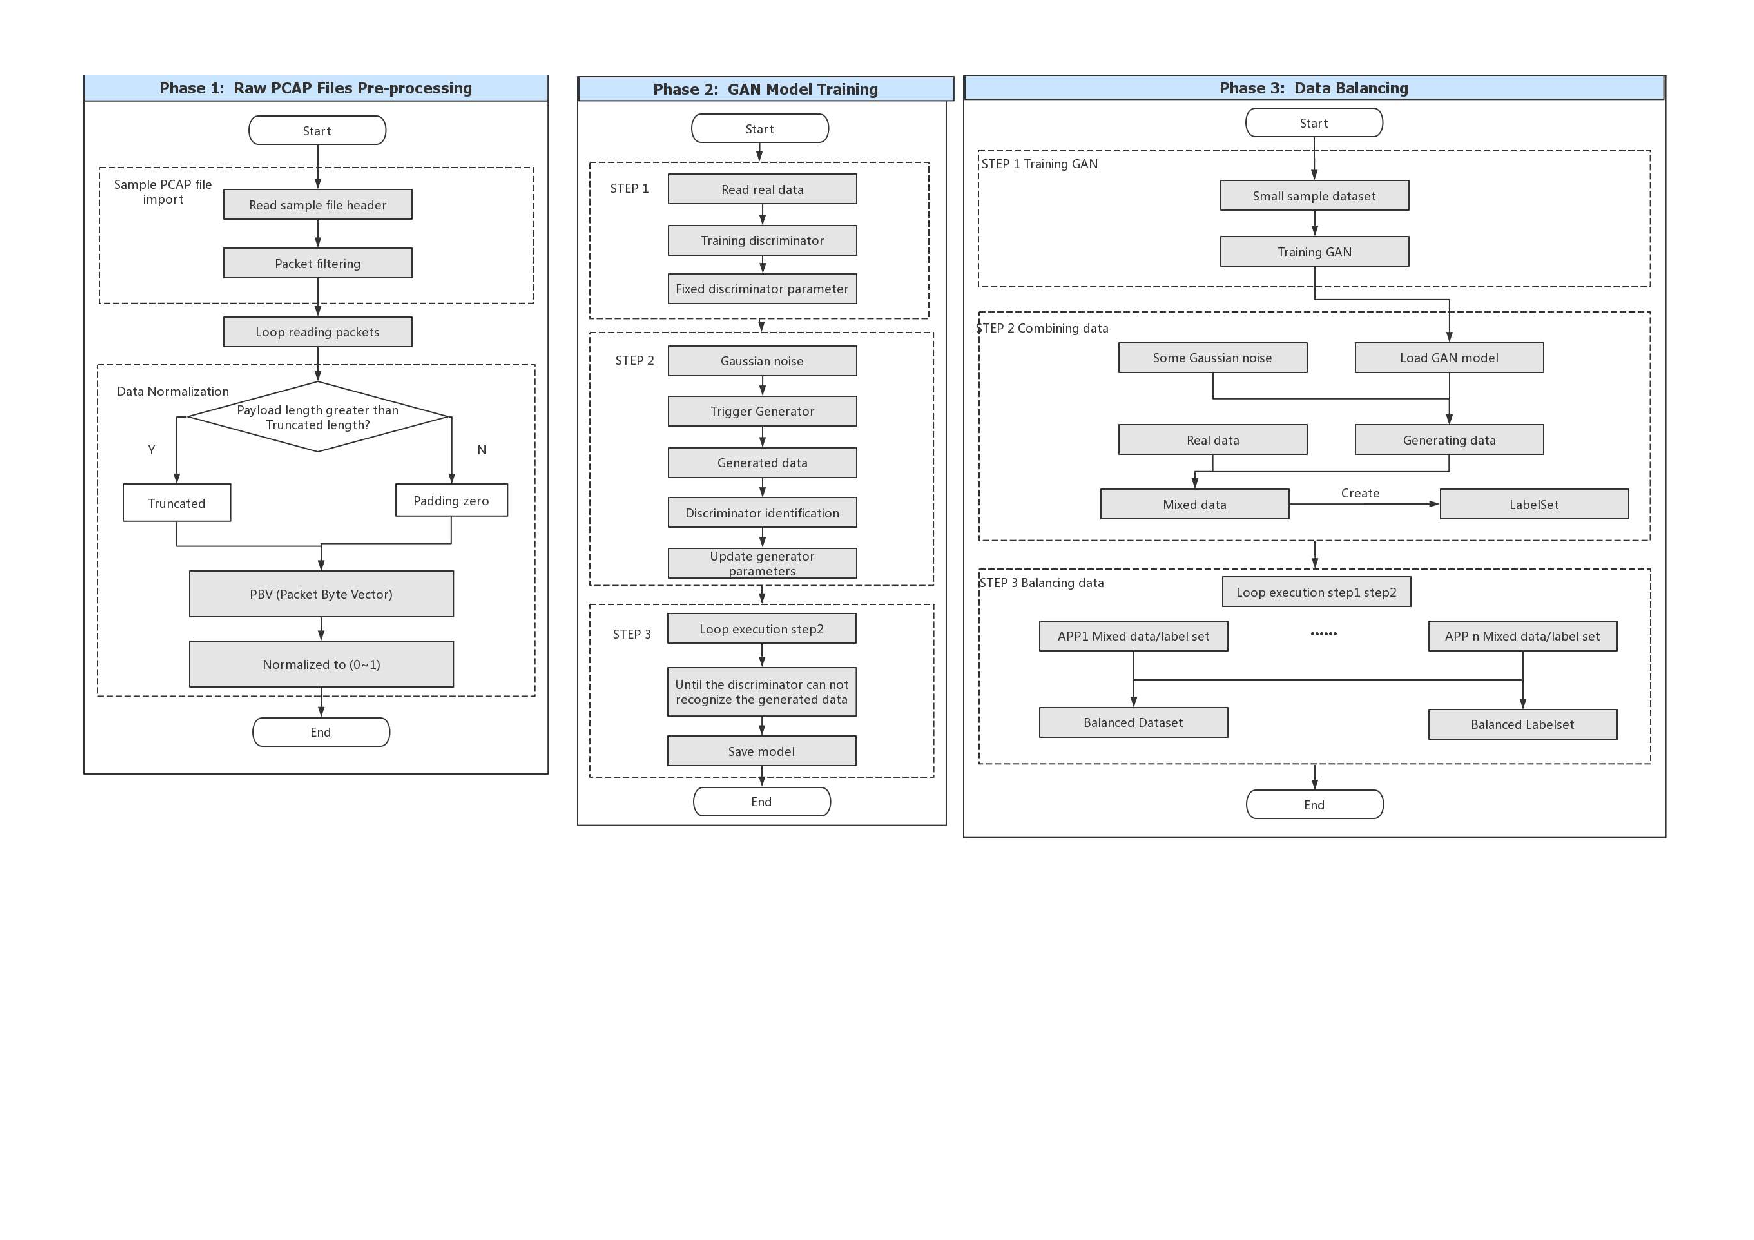
\includegraphics[width=6 in]{figures/Fig_3_flowgan_methodology}
	\caption{The methodology of FlowGAN}
	\label{fig:methodology_gan}
\end{figure}

\subsubsection{Raw PCAP Files Pre-processing}\label{sec:pre-processing}
A raw data packet is always captured in PCAP or PCAPNG format, which has to be pre-processed for the input of subsequent GAN model training. In general, pcap files pre-processing has three steps, \emph{\textbf{filtering}}, \emph{\textbf{truncating/zero padding}} and \emph{\textbf{normalization}}. An overview of the pre-processing procedure (viz. \emph{phase 1}) is shown in Fig.~\ref{fig:methodology_gan}.  \emph{\textbf{filtering}} is to remove the Ethernet header of a raw data packet. Data-link layer information such as MAC address, type of frame, etc., is not useful in packet classification. The \emph{\textbf{filtering}} process reduces the input size of a packet. Moreover, some noise is filtered during the process for better performance. \emph{\textbf{truncating and zero-padding}} is to fix the size of each data packet input to the GAN model. An equal size of all inputs is required for the proposed FlowGAN model. An input after truncating and zero-padding is defined as a Packet Byte Vector (PBV). For example, the $i$-th PBV is described as follows:
\begin{equation}
X_{i} = \{x_{i1}, x_{i2}, x_{i3},....x_{in}\}
\end{equation}
where $x_{ij}$ denotes the $j$-th byte $X_{i}$. Each PBV is then \emph{normalized} to $[0,1]$ for faster convergence. For simplicity, we assume $X_{i}$ is the normalized result of the $i$-th PBV. Generation of a data packet is processed using the normalized PBV. 


\subsubsection{GAN Model Training}
There are three steps during GAN model training. In step 1, the discriminator $D$ is trained with the input of real traffic data from ~\ref{sec:pre-processing} till $D$ is near convergence as shown in Algorithm.~\ref{algorithm:discriminator}. And then step 2 starts while fixing the parameters of $D$, the generator $G$ takes random Gaussian noise as input and generate samples. $D$ receives traffic samples from both the generator and the real traffic data and attempt to distinguish between the two sources as shown in Algorithm.~\ref{algorithm:generator}. These two networks play a competitive game, where the generator is learning to generate more and more realistic traffic samples, and the discriminator is learning to get better and better at distinguishing the generated data from the real data in step 3. These two networks are trained simultaneously, and hope that the competition will drive the generated samples to be indistinguishable from the real data.

To start the training process, training parameters are set as \{$N_e$, $M$, $\eta$\}, where $N_e$ is the maximum number of Epoch, $M$ is the size of mini\_batch used in the stochastic gradient method, $\eta$ is the learning rate. The complete process for the training process is summarized in Algorithm.~\ref{algorithm:discriminator} and ~\ref{algorithm:generator}. Without loss of generality, the algorithm only summarizes the basic structure of the process. Stopping criteria such as validation is not given in the description. 



\begin{algorithm}[ht!]  
	\caption{Discriminator of FlowGAN training}  \label{algorithm:discriminator}
	\begin{algorithmic}[1]  
		\REQUIRE real data from Section ~\ref{sec:pre-processing}
		\ENSURE Discriminator network $D$ of FlowGAN.	
		\FOR {$t=1$ to $N_e$ }
		\FOR {each batch of $M$ input data}
		\STATE For each training samples $X_i \in \mathbb{X}$: 
		\STATE Compute the output using Equation.~(\ref{equ:fake});
		\STATE Process with activation function;
		\STATE Output distinguishing results according to Equation.~(\ref{equ:fake});
		\STATE Compute the training error;
		\STATE Update weights and bias;
		\ENDFOR \\ % end for mini_batch
		\ENDFOR \\ %end for epoch
	\end{algorithmic}  
\end{algorithm}  

\begin{algorithm}[ht!]  
	\caption{Generator of FlowGAN training}  \label{algorithm:generator}
	\begin{algorithmic}[1]  
		\REQUIRE random Guassian noise, fixed discriminator's parameters
		\ENSURE Generator network $G$ of FlowGAN.	
		\FOR {$t=1$ to $N_e$ }
		\FOR {each batch of $M$ input data}
		\STATE For each random Guassian noise input: 
		\STATE Generate the fake synthesized samples as output: 
		\STATE Feed the output samples into discriminator $D$;
		\STATE Process with activation function;
		\STATE Output distinguishing results with the real data according to Equation.~(\ref{equ:fake});
		\STATE Compute the training error;
		\STATE Update weights and bias;
		\ENDFOR \\ % end for mini_batch
		\ENDFOR \\ %end for epoch
	\end{algorithmic}  
\end{algorithm}  



\subsubsection{Data Balancing}
The phase 3 of data balancing is the combination of the training of FlowGAN, mixing the synthesized/real samples and balancing for each class, especially minority class. In our paper, we reduce the size of majority class randomly and augment the size of minority class by FlowGAN.


%Equations are automatically numbered
%\begin{equation}
%f(x) = \alpha \sin (\omega t + \beta) + \gamma
%\label{eq_model}
%\end{equation}

\section{Evaluation and Experimental Results}\label{sec:results}
In this section, we present the experimental results to evaluate the accuracy of the proposed FlowGAN. Moreover, we have to evaluate the performance of FlowGAN by applying the dataset augmented by FlowGAN to the well-known deep learning based network traffic classifier (such as MLP) because there are still no more better quantified performance metrics for GAN.


\subsection{Experiment Settings}\label{sec:expdes}
\subsubsection{Dataset for Evaluation}\label{sec:dataset}

The dataset for evaluation is selected from the ``ISCX VPN-nonVPN traffic dataset''~\cite{ISCX}. As shown in Table~\ref{tab:Desc_Samples}, the total dataset for evaluation is composed of 15 applications, e.g., Facebook, Youtube, Netflix, etc. The chosen applications are encrypted with various security protocols, including HTTPS, SSL, SSH, and proprietary protocols. A total of $206,688$ data packets are included in the selected dataset. Apparently, there are some majority classes like Netflix, which accounts for $25.126\%$ of the total dataset. Accordingly, there are some minority classes like AIM, Email-Client, Facebook, ICQ. To tackle with the imbalance class problem, we further create two datasets with more balanced data samples for each application, which are augmented by the methods of oversampling and FlowGAN respectively. 

%\begin{table}[tp]  
\begin{table}[ht!]	
	\centering  
	\fontsize{6.5}{8}\selectfont  
	\begin{threeparttable}  
		\caption{Description of the chosen datasets.}  \label{tab:Desc_Samples}  
		\begin{tabular}{l|c|cc|cc|cc|}  
			\toprule  
			\multirow{2}{*}{\textbf{Application}}&
			\multirow{2}{*}{\textbf{Security}}&
			\multicolumn{2}{c}{\textbf{Unbalanced dataset}}&\multicolumn{2}{|c}{\textbf{Oversampling  dataset}}&\multicolumn{2}{|c}{\textbf{FlowGAN augmenting dataset}}\cr  
			\cmidrule(lr){3-4} \cmidrule(lr){5-6}\cmidrule(lr){7-8}  
			&\textbf{Protocol} & \textbf{Quantity} & \textbf{Percentage} & \textbf{Quantity} & \textbf{Percentage} & \textbf{Quantity} & \textbf{Percentage}\cr  
			
			\midrule  
			AIM				&HTTPS	 	   &4869&2.356\%	  &10000&6.67\%	  &10067&6.706\%\cr  
			Email-Client&SSL			  &4417&2.137\%		 &10000&6.67\%	 &10015&6.671\%\cr  
			Facebook	&HTTPS	 	   &5527&2.674\%	  &10000&6.67\%	  &10025&6.678\%\cr  
			Gmail		   &HTTPS		  &7329&3.546\%		 &10000&6.67\%	 &10007&6.666\%\cr  
			Hangout		&HTTPS	 	   &7587&3.671\%	  &10000&6.67\%	  &10005&6.664\%\cr  
			ICQ				&HTTPS	 	   &4243&2.053\%	  &10000&6.67\%	  &10001&6.662\%\cr  
			Netflix			&HTTPS		   &51932&25.126\%	&10000&6.67\%	&9999  &6.660\%\cr  
			SCP				&SSH	  		 &15390&7.446\%	   &10000&6.67\%   &9999  &6.660\%\cr  
			SFTP			&SSH	 		 &4729&2.287\%	    &10000&6.67\%	&10007&6.666\%\cr  
			Skype		   &proprietary	 &4607&2.229\%	    &10000&6.67\%	&10005&6.664\%\cr  
			Spotify		   &proprietary	 &14442&6.987\%	   &10000&6.67\%	&9999 &6.660\%\cr  
			torTwitter	  &proprietary	&14654&7.089\%	  &10000&6.67\%	  &9999  &6.660\%\cr  
			Vimeo		  &HTTPS		  &18755&9.074\%	&10000&6.67\%	&9999  &6.660\%\cr  
			voipbuster	&proprietary   &35469&17.161\%	&10000&6.67\%	&9999  &6.660\%\cr  
			Youtube		&HTTPS			 &12738&6.163\%	   &10000&6.67\%   &9999  &6.660\%\cr  							
			\midrule
			
			TOTAL&  &{\bf 206688}&{\bf 100\%}&{\bf 150000}&{\bf 100\%}&{\bf 150125}&{\bf 100\%}\cr  			
			\bottomrule  
		\end{tabular}  
	\end{threeparttable}  
\end{table}  

\subsubsection{Configurations of the Computing Platform}

The performance evaluations are conducted using a Dell R730 server with an Intel I7-7600U CPU \@ 2.8 GHz, 8 GB RAM and an external GPU (Nvidia GeForce GTX 1050TI). The software platform for deep learning is built on Keras library with Tensorflow (GPU-based version 1.9.0) as the back-end support. 

\subsubsection{Description of deep learning based network traffic classifier}
In this paper, we select a well-known deep learning model, Multi-perceptron (MLP) based network traffic classifier to evaluate the performance of our proposed FlowGAN. The MLP network traffic classifier consists of one input layer, two hidden layers and one output layer. Using the full size of the data packet as an example, the input layer has 1480 inputs. The two hidden layers are composed of 6 and 6 neurons respectively. The output layer is composed of 15 neurons with Softmax as classifier. The MLP model has been trained with Adam optimizer and Cross-entropy loss function. 


\subsubsection{Performance Metrics}

The performance metrics used for evaluations of network traffic classifiers are \emph{Precision}, \emph{Recall} and \emph{$F_1$ score}.
\begin{itemize}
	
	\item \textbf{\emph{Precision}}: precision $r_{p}$ is the ratio of \emph{true positives} $n_T^P$ over the sum of $n_T^P$ and \emph{false positives} $n_F^P$. In the proposed classification methods, precision is the percentage of packets that are properly attributed to the targeted application.
	\begin{equation}
	r_p = \frac{n_T^P}{n_T^P+n_F^P}.
	\end{equation}
	
	\item \textbf{\emph{Recall}}: recall $r_c$ is the ratio of $n_T^P$ over the sum of $n_T^P$ and \emph{false negatives} $n_F^N$ or the percentage of packets in an application class that are correctly identified.
	\begin{equation}
	r_c = \frac{n_T^P}{n_T^P+n_F^N}.
	\end{equation}
	
	\item \textbf{\emph{$F_1$-score}}: the $F_1$ score $r_f$ is a widely-used metric in information retrieval and classification that considers both precision and recall as follows:
	\begin{equation}
	r_f = \frac{2 r_p \cdot r_c}{r_p + r_c}.
	\end{equation}
	
\end{itemize}


\subsection{The Performance of FlowGAN}\label{sec:performance_flowgan}
\subsubsection{FlowGAN Model Architecture}
In our experiments, we employ MLP architecture to design Generator and Discriminator network as shown in Table.~\ref{tab:generator_desc} and ~\ref{tab:discriminator_desc}. The input of Generator network is a vector of 100 scalars generated from random Gaussian noise. The following subsequent 3 hidden layers have 128, 256, 512 neurons, respectively and the output layer has 1024 neurons. Accordingly, the input of Discriminator network is the vector of 1024 generated from either real traffic data or output of generator network. Three hidden layers and output layer are all with LeakyReLU as activation function. During the process of training for FlowGAN, we take Adam as optimizer and cross-entropy as loss function with 1000 epoches and 256 of mini\_batch.

\begin{table}[ht!]	
	\centering  
	\fontsize{6.5}{8}\selectfont  
	\begin{threeparttable}  
		\caption{Generator model description of FlowGAN.}  \label{tab:generator_desc} 
			\begin{tabular}{cc|cc|cc|cc|cc}  
			\toprule  
			\multicolumn{2}{c}{\textbf{Input Layer}}&\multicolumn{2}{|c}{\textbf{Hidden Layer1}}&\multicolumn{2}{|c}{\textbf{Hidden Layer 2}}&\multicolumn{2}{|c}{\textbf{Hidden Layer 3}}&\multicolumn{2}{|c}{\textbf{Output Layer}}\cr  
			\cmidrule(lr){1-2}\cmidrule(lr){3-4} \cmidrule(lr){5-6}\cmidrule(lr){7-8} \cmidrule(lr){9-10}
			\textbf{Input} &\textbf{Activation} & \textbf{Output} & \textbf{Activation} & \textbf{Output} & \textbf{Activation} & \textbf{Output} & \textbf{Activation} & \textbf{Output} & \textbf{Activation}\cr  

			\midrule  
			100& LeakyReLU &128				&LeakyReLU	 	   &256&LeakyReLU	  &512&LeakyReLU	  &1024&LeakyReLU\cr  
			\midrule

		\end{tabular}  
	\end{threeparttable}  
\end{table}  


\begin{table}[ht!]	
	\centering  
	\fontsize{6.5}{8}\selectfont  
	\begin{threeparttable}  
		\caption{Discriminator model description of FlowGAN.}  \label{tab:discriminator_desc}  
		\begin{tabular}{cc|cc|cc|cc|cc}  
			\toprule  
			\multicolumn{2}{c}{\textbf{Input Layer}}&\multicolumn{2}{|c}{\textbf{Hidden Layer1}}&\multicolumn{2}{|c}{\textbf{Hidden Layer 2}}&\multicolumn{2}{|c}{\textbf{Hidden Layer 3}}&\multicolumn{2}{|c}{\textbf{Output Layer}}\cr  
			\cmidrule(lr){1-2}\cmidrule(lr){3-4} \cmidrule(lr){5-6}\cmidrule(lr){7-8} \cmidrule(lr){9-10}
			\textbf{Input} &\textbf{Activation} & \textbf{Output} & \textbf{Activation} & \textbf{Output} & \textbf{Activation} & \textbf{Output} & \textbf{Activation} & \textbf{Output} & \textbf{Activation}\cr  
			
			\midrule  
			1024& LeakyReLU &512				&LeakyReLU	 	   &256&LeakyReLU	  &128&LeakyReLU	  &1&Softmax\cr  
			\midrule
			
		\end{tabular}  
	\end{threeparttable}  
\end{table}  



\subsubsection{Loss of Generator and Discriminator Network of FlowGAN}
As shown in Fig.~\ref{fig:loss_flowgan}, training loss of FlowGAN over three minority application classes are demonstrated, which are aim\_chat, ICQ\_chat, hangout\_chat. Apparently, discriminator is fitted stably after 100 epoches, on the contrary, generator after 600 epoches.    

\begin{figure*}[ht!]
	\centering
	%	\vspace*{-3mm}
	\subfigure[Loss of aim\_chat.]{\label{fig:CM-MLP-im-Avedata}
		\begin{minipage}[c]{0.33\textwidth}
			\centering
			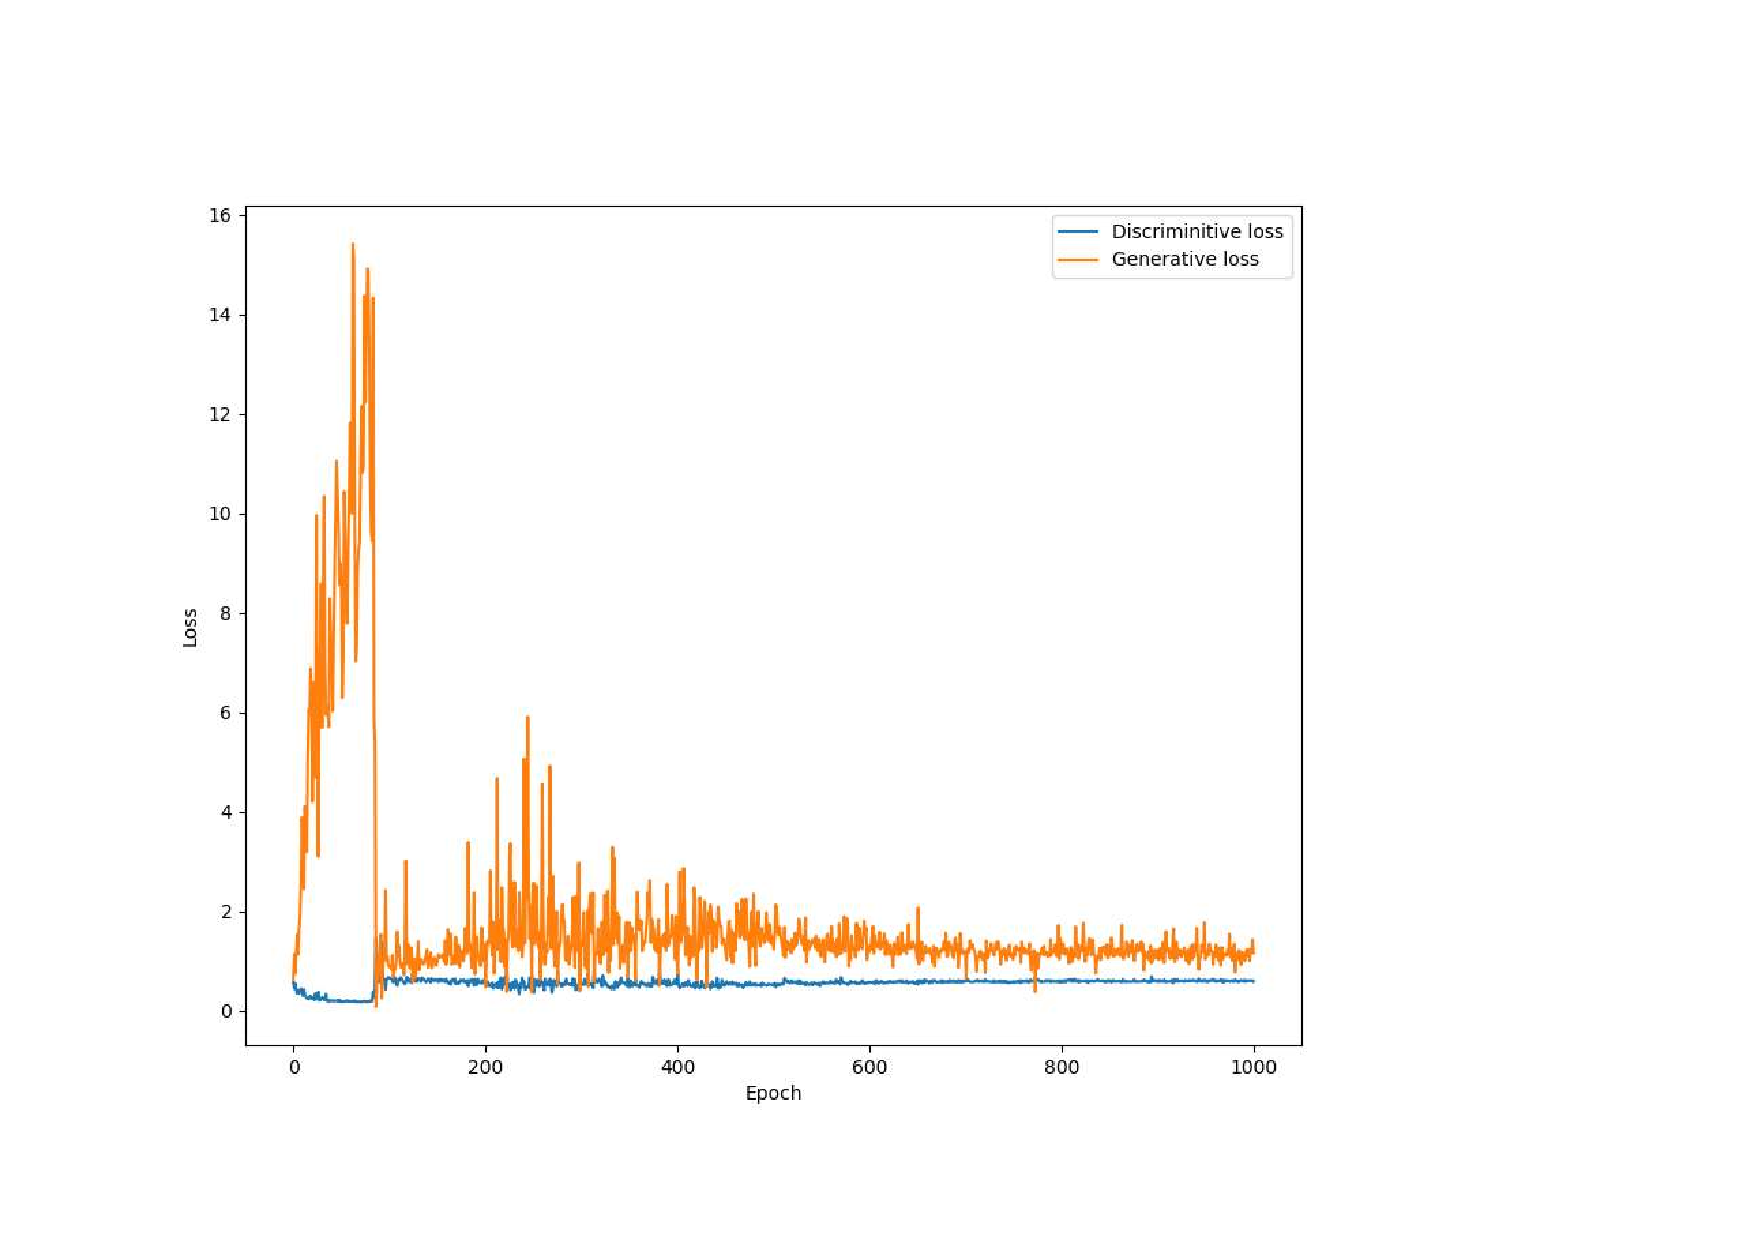
\includegraphics[width=2.3 in]{figures/AIM_chats_gan_loss}
		\end{minipage}%
	}%
	\centering
	%	\vspace*{-3mm}
	\subfigure[Loss of ICQ\_chat.]{\label{fig:CM-SAE-im-Avedata}
		\begin{minipage}[c]{0.33\textwidth}
			\centering
			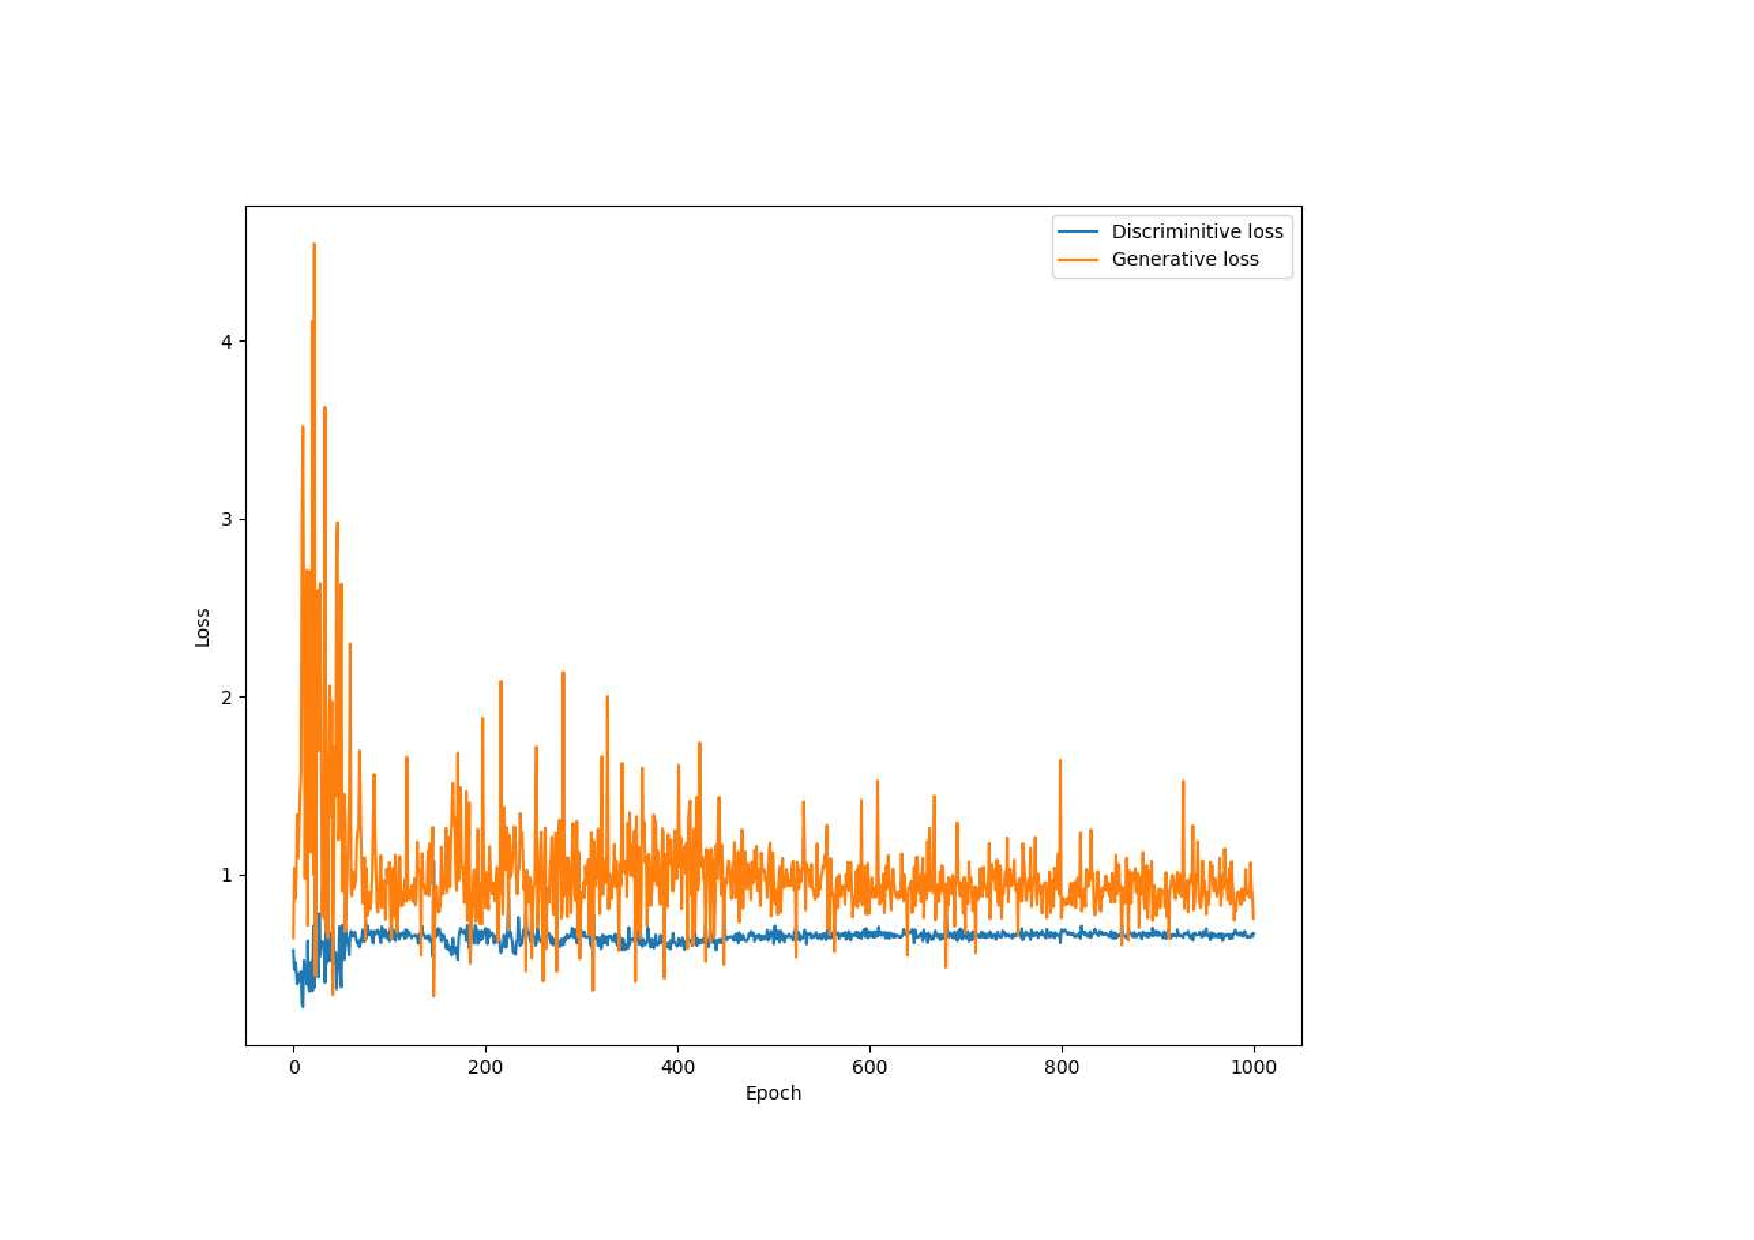
\includegraphics[width=2.3 in]{figures/ICQ_chats_gan_loss}
		\end{minipage}%
	}%
	\centering
	\subfigure[Loss of hangout\_chat.]{\label{fig:CM-CNN-im-Avedata}
		\begin{minipage}[c]{0.33\textwidth}
			\centering
			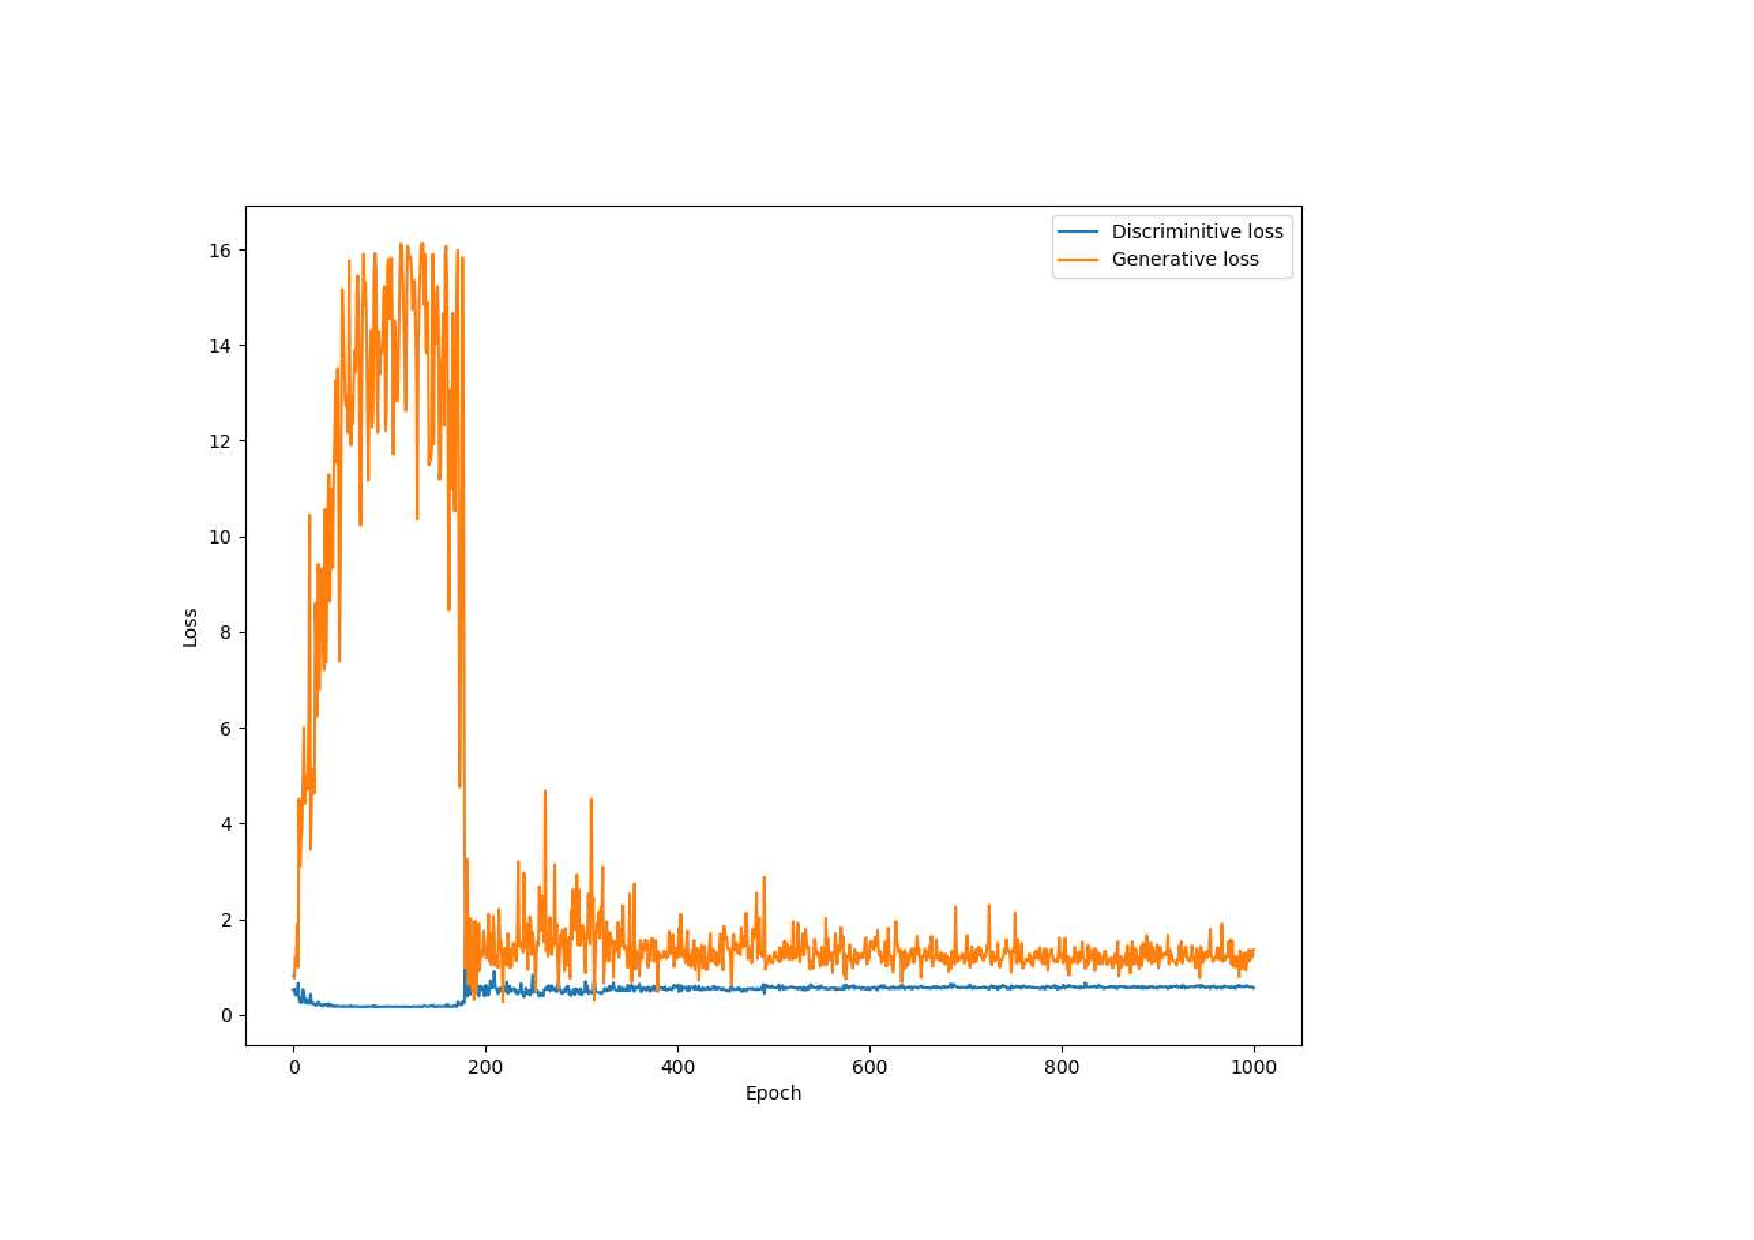
\includegraphics[width=2.3 in]{figures/hangout_chat_4b_gan_loss}
		\end{minipage}%
	}	\caption{Loss of FlowGAN (three minority classes from 15 applications).}\label{fig:loss_flowgan}
	%	\vspace*{-3mm}
\end{figure*}




\subsection{The performance of MLP-based Network Traffic Classifier}
From the Table.~\ref{table:performance_classifier}, we can see that MLP classifier on FlowGAN dataset outperforms the other two methods about Accuracy, Precision, Recall and F1-Score. Furthermore, we can verify that FlowGAN can properly improve the problem of class imbalance and get better performance than oversampling method. 
\begin{table}[ht!]
	\centering
	\caption{Performance of MLP-based traffic classifier.}\label{table:performance_classifier}
	\begin{tabular}{|c|c|c|c|c|}% left center and right.
		\hline
		data augmenting methods & Accuracy & Precision & Recall & F1-Score \\
		\hline
		\textbf{MLP classifier on unbalanced dataset}  & 0.8995 & 0.9 & 0.8995 &  0.8968 \\
		\hline
		\textbf{MLP classifier on oversampling dataset}   & 0.9794 & 0.9799 & 0.9794& 0.9796 \\
		\hline
		\textbf{MLP classifier on FlowGAN dataset}   & 0.991 & 0.9911 & 0.991  & 0.991 \\
		\hline
	\end{tabular}
\end{table}



\begin{figure*}[ht!]
	\centering
	%	\vspace*{-3mm}
	\subfigure[Precision of MLP based classifier.]{\label{fig:precision_compare}
		\begin{minipage}[c]{0.33\textwidth}
			\centering
			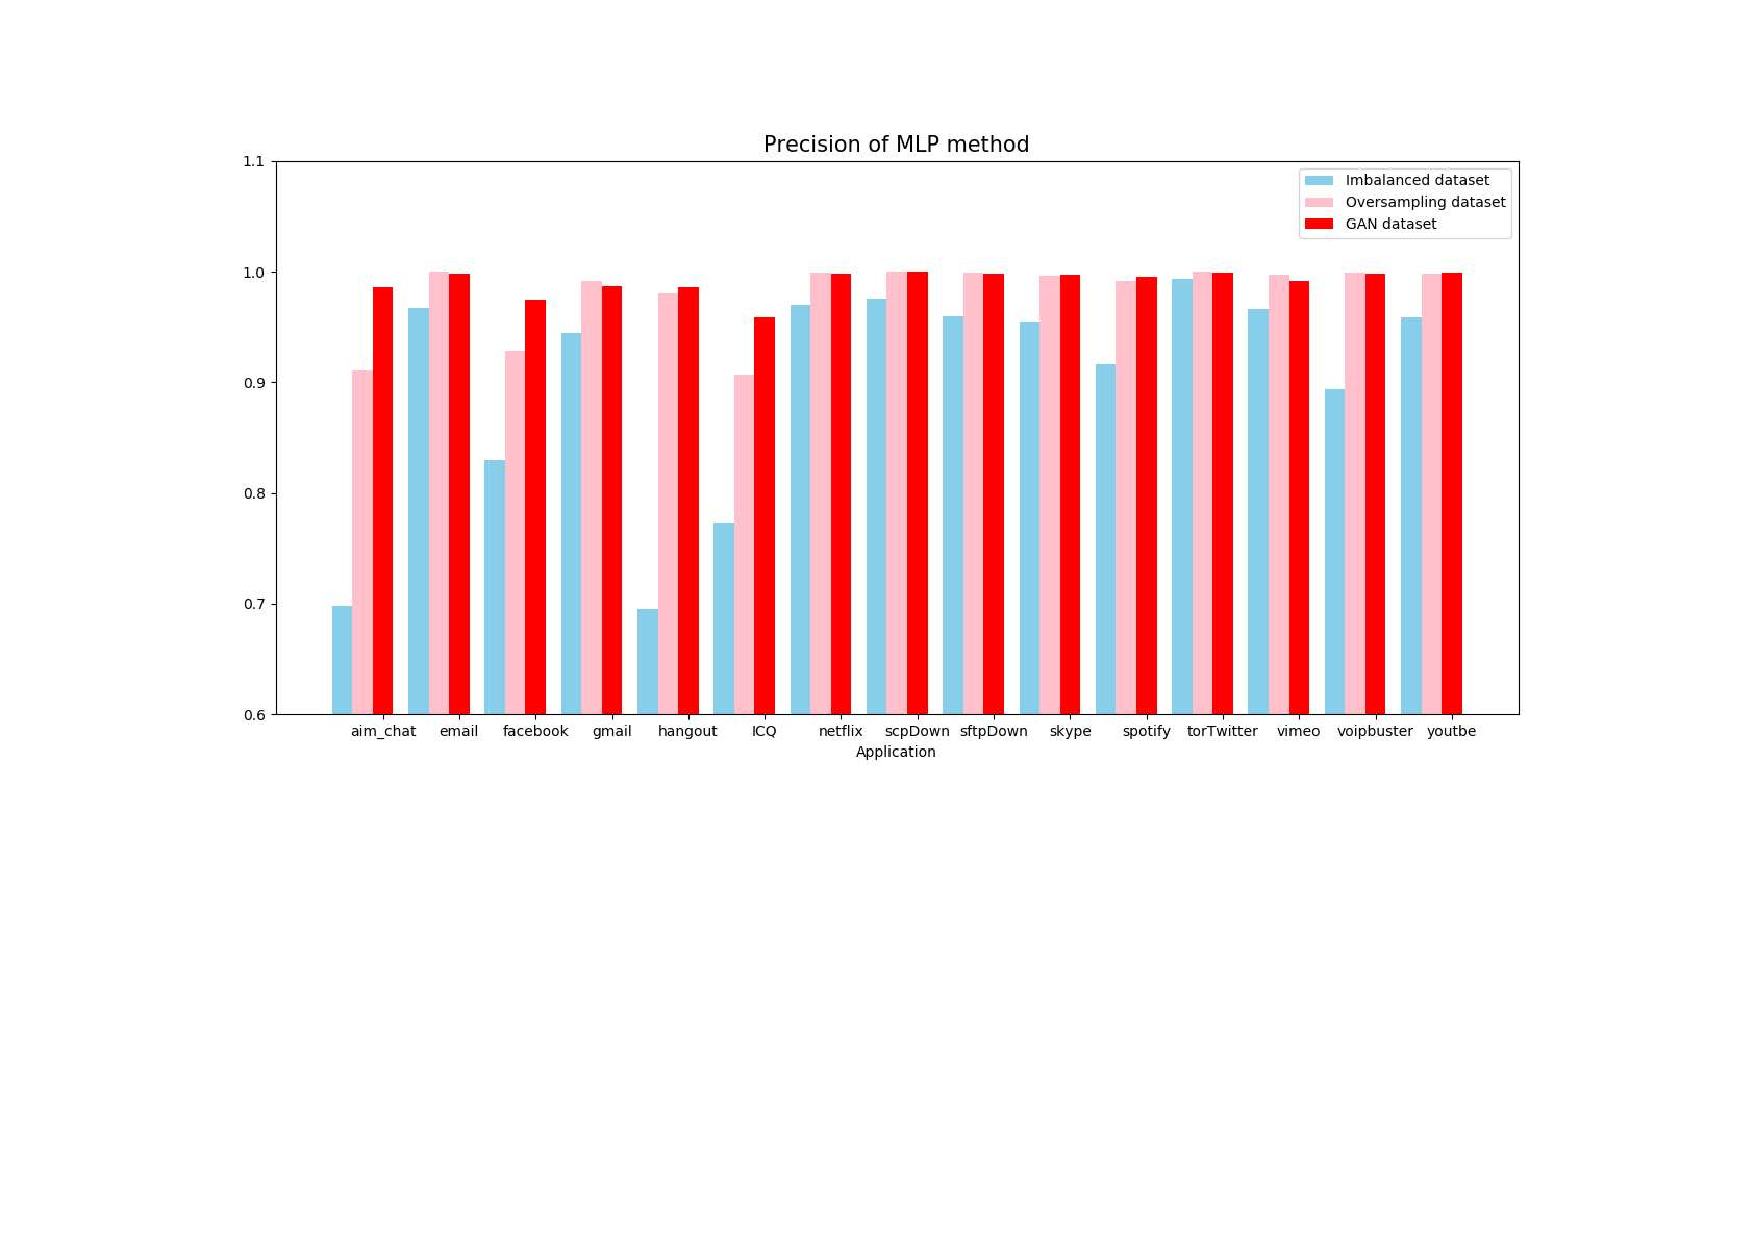
\includegraphics[width=2.3 in]{figures/Precision-compare}
		\end{minipage}%
	}%
	\centering
	%	\vspace*{-3mm}
	\subfigure[Recall of MLP based classifier.]{\label{fig:recall_compare}
		\begin{minipage}[c]{0.33\textwidth}
			\centering
			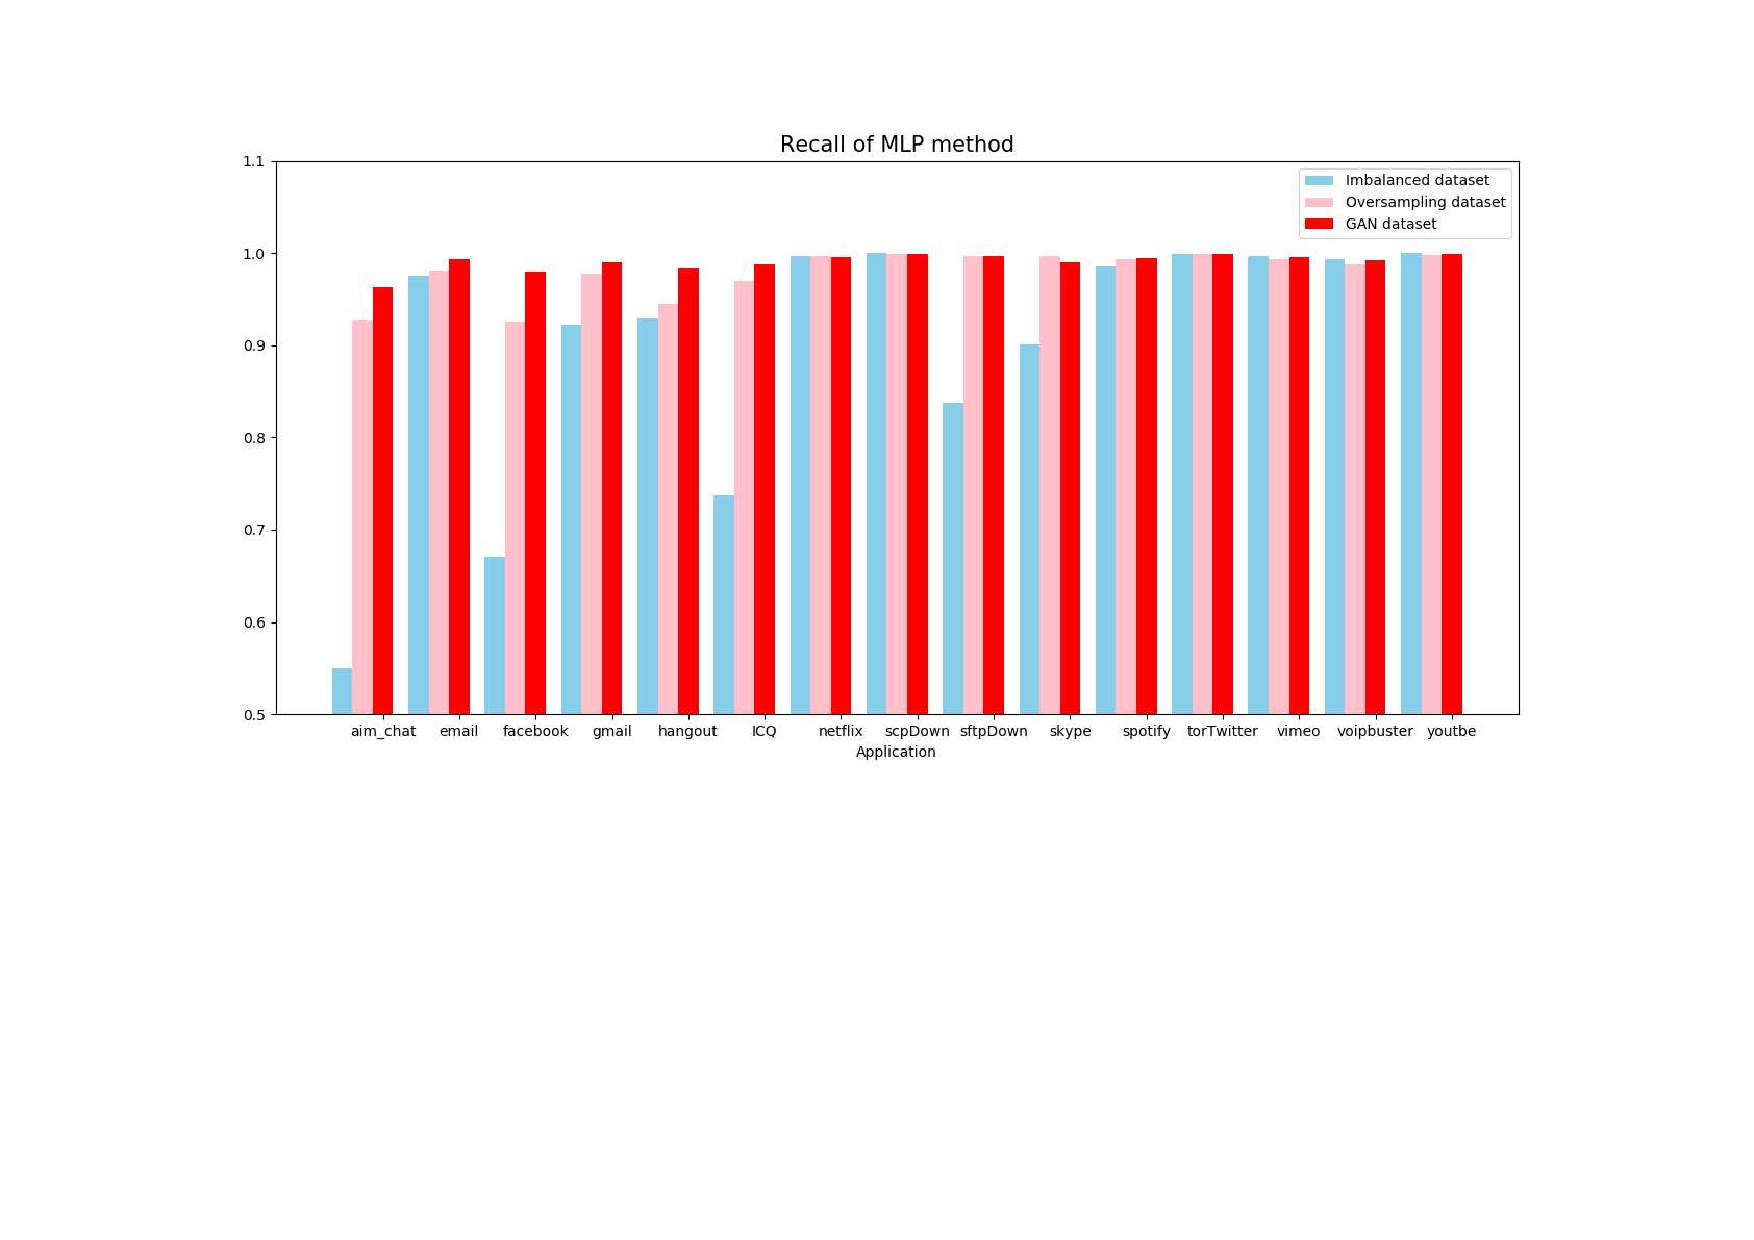
\includegraphics[width=2.3 in]{figures/Recall-compare}
		\end{minipage}%
	}%
	\centering
	\subfigure[F1-Score of MLP based classifier.]{\label{fig:f1-compare}
		\begin{minipage}[c]{0.33\textwidth}
			\centering
			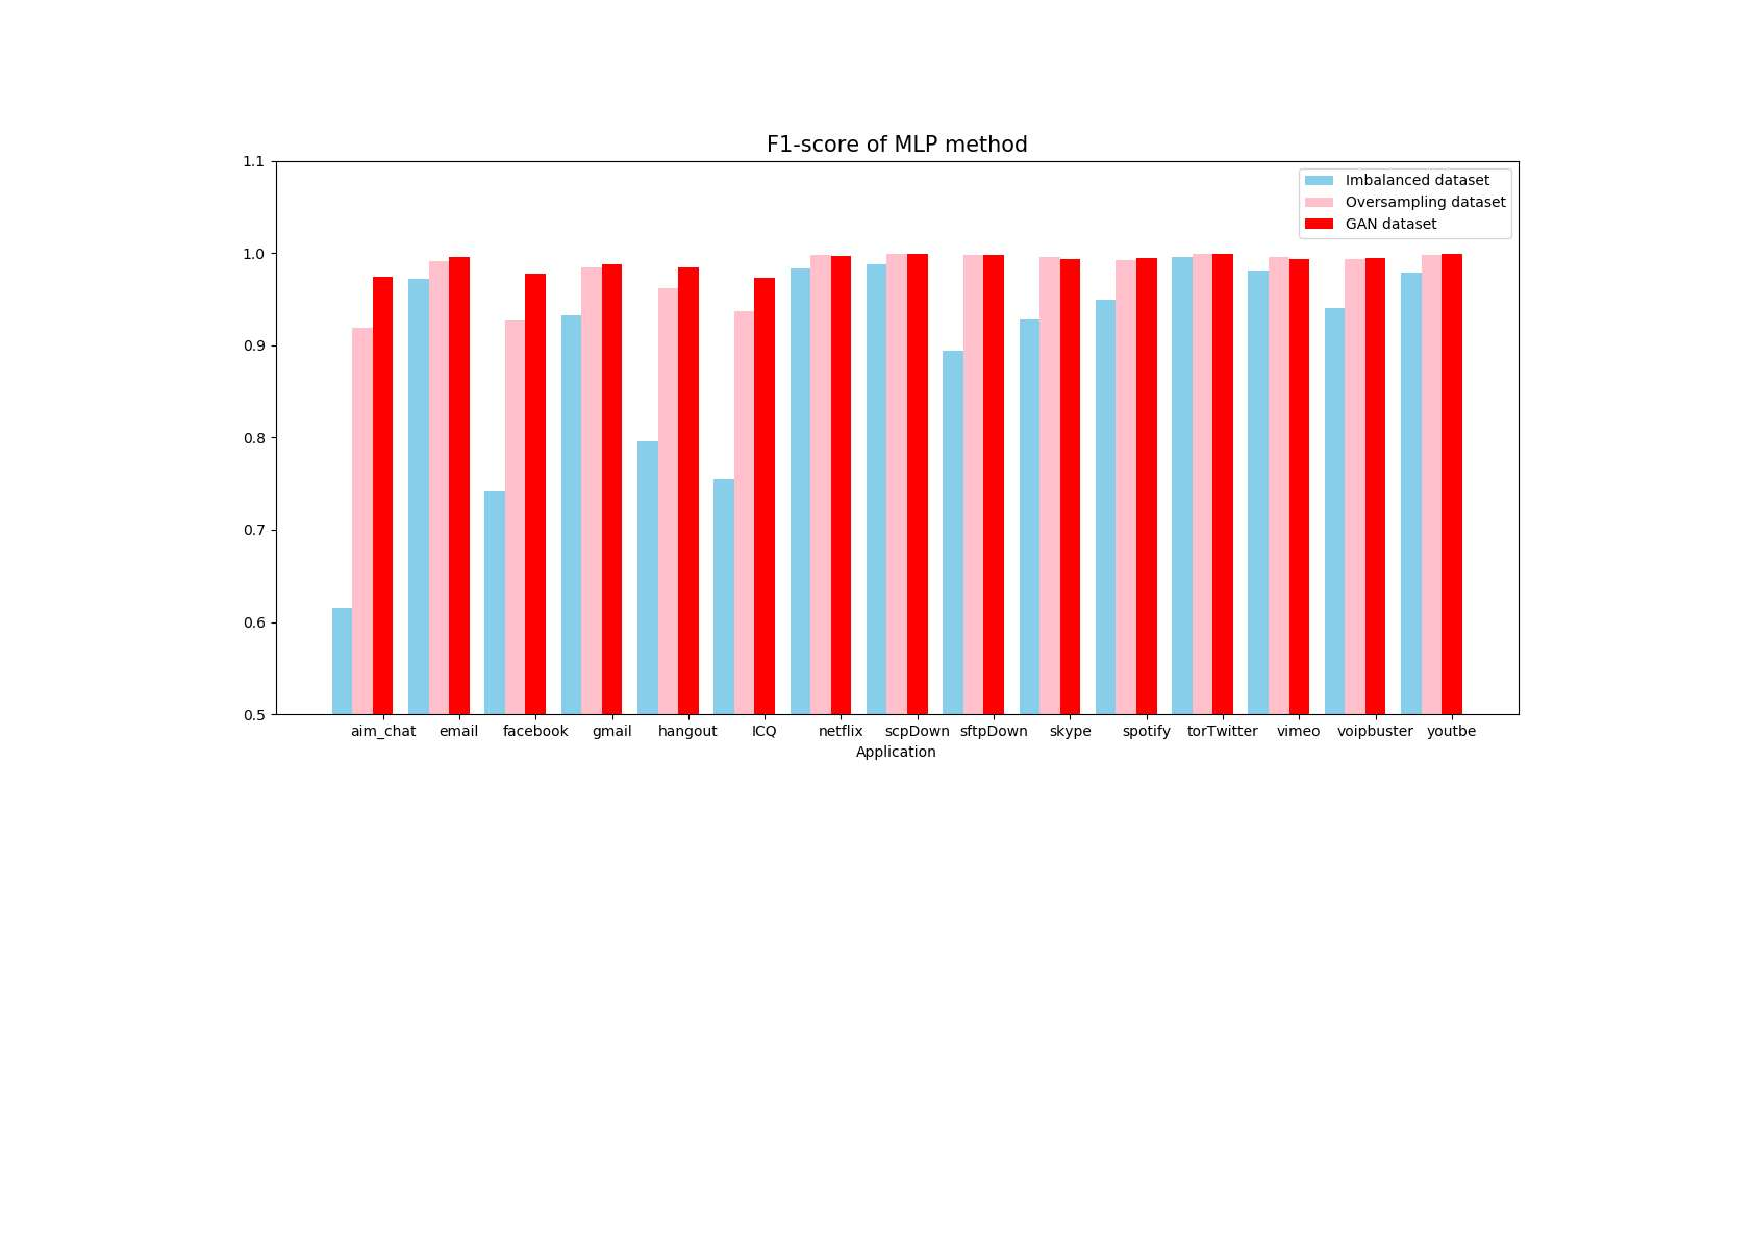
\includegraphics[width=2.3 in]{figures/F1-compare}
		\end{minipage}%
	}	\caption{Performance comparison between three methods.}\label{fig:performance_comparison}
	%	\vspace*{-3mm}
\end{figure*}











\section{Conclusion and Future work}
In this paper, we proposed the design and development of Generative Adversarial Network (GAN) based traffic data augmenting method called FlowGAN to generate synthesized samples for encrypted traffic classification. The synthesized data is then combined with the original (viz. real) data to construct the new traffic training dataset. As a proof of concept, we adopted three state-of-the-art deep learning based encrypted traffic classification methods, MLP on our new augmented training dataset synthesized from our FlowGAN. The experimental results demonstrate that our proposed FlowGAN can achieve better performance compared with  other traditional data augmenting methods like over sampling. In the future, we will further study the other genre of GAN, like CGAN, WGAN for traffic classification to improve the performance of data augmentation methods.


\vspace{2ex}
\noindent
{\bf\normalsize Acknowledgement}\newline
{The authors would like to thank the hardworking effort of my postgraduates for the experiments of FlowGAN.}

% Reference
% Please update the Reference.bib
\renewcommand\refname{Reference}
\bibliographystyle{IEEEtran}
\bibliography{IEEEfull,Reference}

%\bibliographystyle{IEEEtran}
%Bibliography file should be compiled with BibTex
%\bibliography{Bibli2}
\noindent
{\bf\normalsize Biography}


\begin{figure}[ht!]
	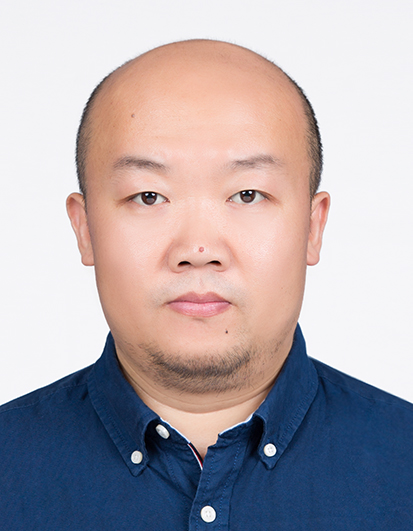
\includegraphics[width=1 in]{figures/wp} 
\end{figure}

\noindent{\it Pan Wang} (M'18) received the BS degree from the Department of Communication Engineering, Nanjing University of Posts \& Telecommunications, Nanjing, China, in 2001, and the PhD degree in Electrical \& Computer Engineering from Nanjing University of Posts \& Telecommunications, Nanjing, China, in 2013. He is currently an Associate Professor in the School of Modern Posts, Nanjing University of Posts \& Telecommunications, Nanjing, China. His research interests include cyber security and communication network security, network measurements, Quality of Service, Deep Packet Inspection, SDN, big data analytics and applications. From 2017 to 2018, he was a visiting scholar of University of Dayton (UD) in the Department of Electrical and Computer Engineering.(email:wangpan@njupt.edu.cn)

\begin{figure}[ht!]
	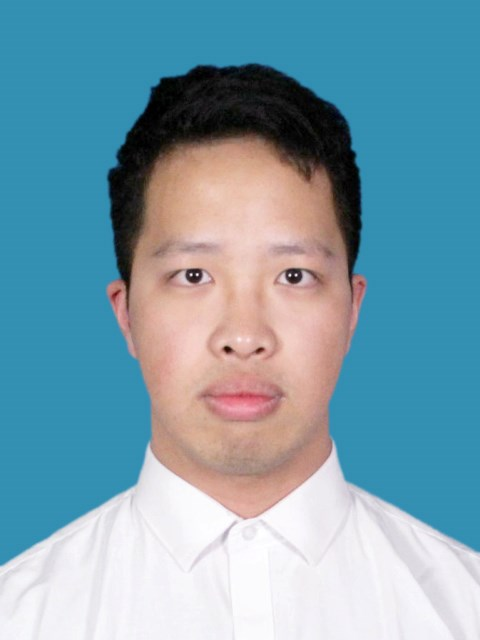
\includegraphics[width=1 in]{figures/wzx} 
\end{figure}

\noindent{\it ZiXuan Wang} was born in Nanjing, Jiangsu, China ,in 1994 . He obtained a bachelor's degree from Tongda College of Nanjing University of Posts and Telecommunications in 2017, He is currently pursuing a master's degree in logistics engineering at Nanjing University of Posts and Telecommunications, under the direction of Professor Wang. His research interests include encrypted traffic identification and data balancing.(email:wangzx@runtrend.com.cn)

\begin{figure}[ht!]
	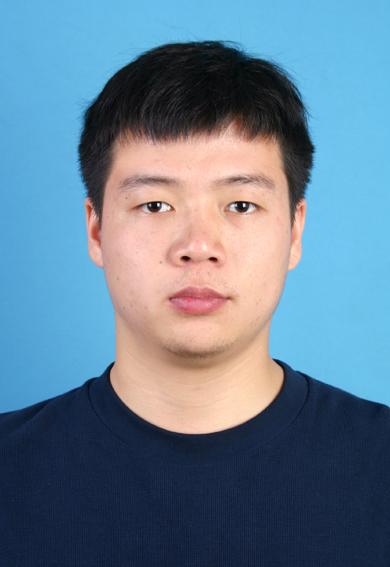
\includegraphics[width=1 in]{figures/li} 
\end{figure}
\noindent{\it ShuHang Li} was graduated from Jiangsu University of Science and Technology,Zhenjiang ,China, in 2013.He is currently pursuing a master's degree at Nanjing University of Posts \& Telecommunications,Nanjing China.His research direction is encrypted traffic identification,and he also interested in Deep Packet Inspection and applications.(email:lish@runtrend.com.cn)


\begin{figure}[ht!]
	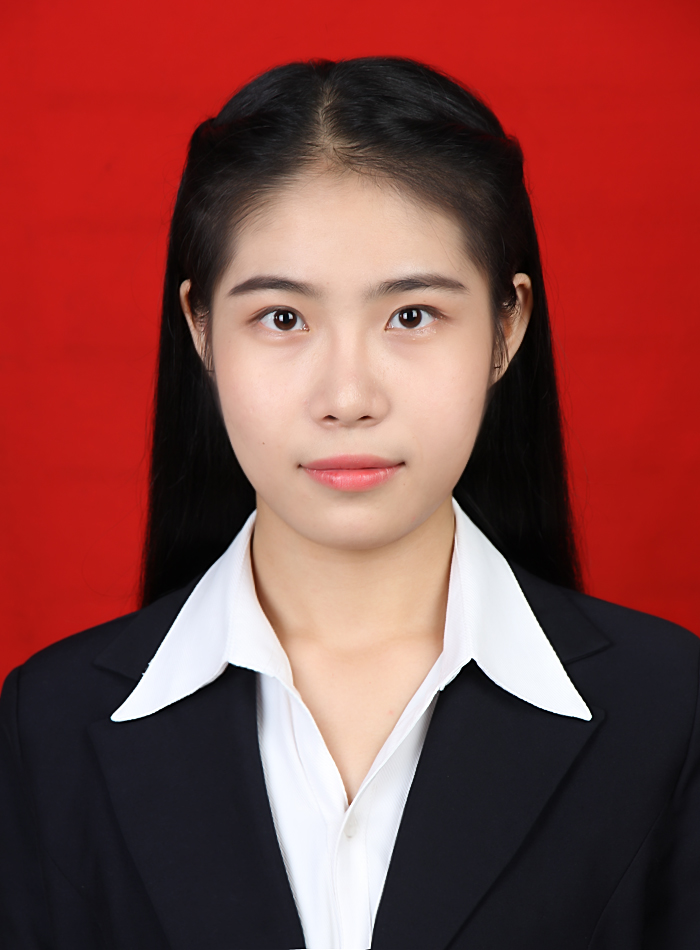
\includegraphics[width=1 in]{figures/huang} 
\end{figure}
\noindent{\it Chen Huang} was born in Xi'an, Shaanxi, China, in 1995. She received the B.S. degree from School of Communication and Information Technology, Xi'an University of Posts \& Telecommunications, in 2017. She is currently pursuing the master's degree in logistics engineering with the Nanjing University of Posts and Telecommunications, under the supervision of Prof. P. Wang. His research interests include data mining and recommendation systems.(email: ahchenen@163.com)

\begin{figure}[ht!]
	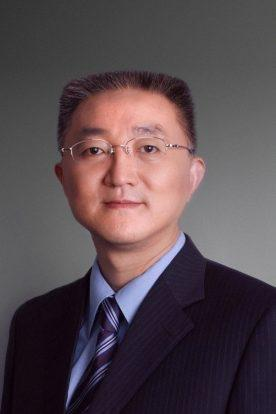
\includegraphics[width=1 in]{figures/feng} 
\end{figure}
\noindent{\it Feng Xiang} received his B.A. degree from Nanjing University and Master of Public Administration from JFK School of Government, Harvard University. He is currently CEO of YTO Express Company Ltd and Director of National Engineering Laboratory for Logistics Information Technology. His research interests include logistics engineering and strategic management of business.(email: 13770610203@163.com)

\end{document}


